% Chapter 1

\chapter{Introducción general} % Main chapter title

\label{Chapter1} % For referencing the chapter elsewhere, use \ref{Chapter1} 
\label{IntroGeneral}
En este capítulo se presenta una introducción técnica a Internet de las cosas y se describen la motivación, algunos sistemas comerciales del mercado, los objetivos y el alcance del presente trabajo.
%----------------------------------------------------------------------------------------

% Define some commands to keep the formatting separated from the content 
\newcommand{\keyword}[1]{\textbf{#1}}
\newcommand{\tabhead}[1]{\textbf{#1}}
\newcommand{\code}[1]{\texttt{#1}}
\newcommand{\file}[1]{\texttt{\bfseries#1}}
\newcommand{\option}[1]{\texttt{\itshape#1}}
\newcommand{\grados}{$^{\circ}$}

%----------------------------------------------------------------------------------------

%\section{Introducción}

%----------------------------------------------------------------------------------------

%\section{Conceptos generales}

%En esta sección se describen aspectos esenciales para poder conocer y entender las tecnologías %y servicios usados en el trabajo.

\section{IoT y computación en la nube}

Internet de las cosas (IoT) y la computación en la nube (\emph{Cloud Computing}) son dos conceptos y soluciones que cada día ocupan una mayor importancia en el desarrollo tecnológico industrial y empresarial, pero antes de abordar su rol es importante definirlos:

\begin{itemize}
\item Internet de las cosas (IoT): hace referencia a una tecnología basada en la conexión de objetos cotidianos a Internet que intercambian, agregan y procesan información sobre su entorno físico para proporcionar servicios de valor añadido a los usuarios finales. También reconoce eventos o cambios, y tales sistemas pueden reaccionar de forma autónoma y adecuada \citep{BOOK:1}.

IoT es un conjunto de tecnologías que facilita la integración de sensores y actuadores que informan del estado de elementos, como electrodomésticos, vehículos, herramientas o incluso seres vivos y permite la conectividad con plataformas en la nube que reciben y procesan la información.

\item \emph{Cloud Computing}: la computación en la nube como paradigma proporciona a las empresas y usuarios soluciones informáticas (como \emph{software}, almacenamiento de datos, capacidad de procesamiento, etc.) a través de Internet que son fácilmente escalables bajo demanda. Los documentos, correos electrónicos y otros datos, así como las aplicaciones informáticas, se almacenarán ``en la nube'', es decir, en línea, de modo que se puede acceder a los mismos desde cualquier ordenador o dispositivo móvil \citep{BOOK:1}.

La generalización del \emph{Cloud Computing} en la infraestructura TIC (tecnologías de información y comunicación) habilita la viabilidad de ejecutar aplicaciones completamente en Internet. En particular, aumenta la flexibilidad en el acceso \citep{BOOK:1}.

%La computación en la nube es una tecnología que permite acceso a \emph{software}, almacenaje de ficheros y procesamiento de datos a través de Internet, siendo una opción alternativa a la ejecución en un servidor local. 

En el modelo de nube, no es necesario instalar aplicaciones de forma local en computadoras.

\end{itemize}

\section{Sensores y redes inalámbricas}

En la revolución de la industria conectada (Industria 4.0) \citep{WEBSITE:31}  cada vez existe una mayor oferta de sensores inteligentes que, además de medir la magnitud en cuestión, llevan integrado un circuito electrónico compatible con los estándares de comunicaciones más habituales en el mundo de IoT. Para lograr dicha tarea es necesario la interacción de dos elementos principales:

\begin{itemize}
\item Sensores: permiten llevar la realidad a una dimensión que se pueda gestionar para finalmente tomar decisiones e, incluso, actuar sobre el propio entorno. Los sensores convierten la magnitud de entrada (temperatura, humedad, nivel, presión, etc.) en una señal eléctrica medible e interpretable por dispositivos electrónicos.

\item Redes inalámbricas (\emph{Wireless}): logran propagar la conexión entre dispositivos a través de medios no físicos. Usan diferentes tecnologías como ondas electromagnéticas, radiación y medios ópticos para su transferencia. Existen varios tipos de redes inalámbricas con diferentes alcances y funcionalidades tales como: redes de corto alcance y bajo consumo y redes de área extensa de bajo consumo \citep{WEBSITE:15}. La distancia a la que los datos deben viajar (corta o larga) determina el tipo de conectividad necesaria para un proyecto de IoT.

\end{itemize}

%\section{Tipos de redes de IoT}

%Podemos clasificarlas en dos categorías:
%\begin{enumerate}
%\item Redes de corto alcance y bajo consumo 

%Las redes de baja potencia y corto alcance están indicadas para hogares, oficinas y otros %entornos de reducido tamaño. Normalmente, necesitan baterías pequeñas y su uso suele resultar %económico \citep{WEBSITE:15}. Por ejemplo:

%\begin{itemize}
%\item Bluetooth
%\item Z-Wave
%\item NFC
%\item ZigBee
%\item Wi-Fi/802.11
%\end{itemize}

%\vspace{1cm}

%\item Redes de área extensa de bajo consumo (LPWAN)

%Las redes LPWAN permiten la comunicación en un radio mínimo de 500 metros, tienen un consumo de energía mínimo y se usan para la mayoría de los dispositivos IoT \citep{WEBSITE:15}. 

%Los siguientes son algunos ejemplos comunes de redes LPWAN:

%\begin{itemize}
%\item 4G LTE para IoT
%\item 5G para IoT
%\item Cat-0
%\item Cat-1
%\item LoRaWAN
%\item LTE Cat-M1
%\item Sigfox
%\item Banda estrecha o NB-IoT/Cat-M2
%\end{itemize}

%\end{enumerate}

%\vspace{0.5cm}



\section{Sistema de gestión de edificios}
Los \emph{Building Management Systems} (BMS), o sistemas de gestión de edificios, son usados en todo tipo de inmuebles públicos y privados. Su función es mejorar la gestión y control, avanzando hacia el concepto de ``edificio inteligente''. Estos sistemas emplean procedimientos automatizados que funcionan para regular y controlar los sistemas esenciales del edificio, que incluyen: calefacción, ventilación y aire acondicionado, iluminación, energía, uso de servicios públicos y CCTV (\emph{Closed Circuit Television}). Para lograr la integración y comunicación entre componentes se requiere \emph{software} y \emph{hardware} que pueda coordinar, monitorear y controlar a través de la red del edificio. La figura \ref{fig:bms}  ilustra los componentes que tiene un sistema BMS.

La combinación de las soluciones de BMS con nuevas tecnologías como el Big Data, IoT, el aprendizaje automático o la inteligencia artificial permiten que un edificio no solo sea más fácil de mantener, sino que pueda llegar a autogestionarse de acuerdo con los parámetros definidos por sus responsables. Entre las principales ventajas de un sistema BMS se consideran:

\vspace{0.25cm}
\begin{itemize}
\item Permite el control y supervisión centralizados de todos los elementos del edificio.
\item Facilita la rápida detección de las incidencias para un mantenimiento preventivo.
\item Proporciona información detallada del consumo que fomenta la eficiencia energética.
\item La mejora de la gestión incrementa el confort y seguridad de los usuarios del edificio.
\end{itemize} 


\begin{figure}[htbp]
\centering
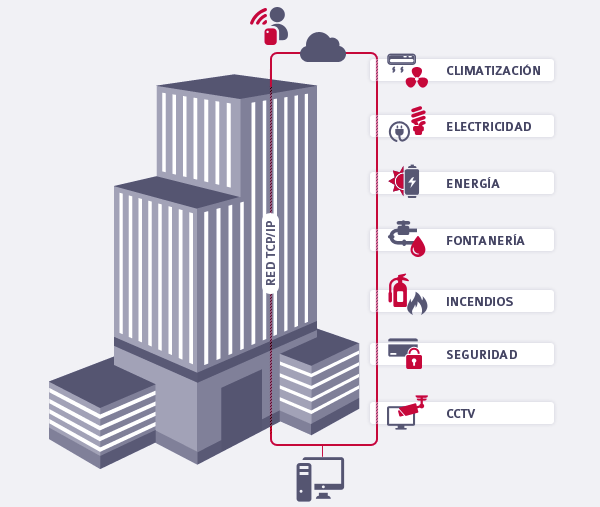
\includegraphics[width=.9\textwidth]{./Figures/bms2.png}
\caption{Componentes de un sistema de gestión de edificios \protect\footnotemark .}
\label{fig:bms}
\end{figure}

\footnotetext{Imagen tomada de \url{https://n9.cl/sistemas_bms}}

\section{Estado del arte}
En la actualidad existe una amplia variedad de sistemas relacionados a los BMS ofrecidos por empresas multinacionales como ENERGY MANAGER de la empresa \emph{Honeywell International Inc} \citep{WEBSITE:35}, IAMMETER de la empresa \emph{Beijing Lewei IOT Technologies Co. Ltd.} \citep{WEBSITE:36} y BEE2ENERGY de la empresa \emph{Compta Energing Business} \citep{WEBSITE:37}. Estos sistemas, presentan facilidad a la hora de integrar nuevos dispositivos a la red (\emph{Ethernet} o \emph{Wireless}) preexistente y suelen enfocarse en algunas de las variables a supervisar en el edificio, como la gestión de la energía eléctrica como objetivo principal. Estos sistemas fueron tenidos en cuenta para la toma de decisiones entorno al desarrollo del proyecto, y por ello se resumen algunas características de estos en las tablas \ref{tab:tabla2} y \ref{tab:tabla3}:


%%%%%%%%%%%%%%%%%%%%%%%%%%%%%%%%%%%%%%
%escribir texto 2

\begin{table}[h]
	\centering
	\caption[Comparativa de soluciones entre acceso y servidor]{Comparativa acceso y tipo de servidor.}
	\begin{tabular}{l c c c c }    
		\toprule
		\textbf{Producto} & \textbf{Acceso}  & \textbf{Uso} & \textbf{S. local}   & \textbf{S. remoto} \\
		\midrule
		Energy Manager & local y remoto 	& navegador & no & sí  \\		
		Iammeter	 & local y remoto	& navegador y app. & no & sí  \\
		Bee2energy	 & local y remoto	& navegador & no & sí  \\
		\bottomrule
		\hline
	\end{tabular}
	\label{tab:tabla2}
\end{table}

%\vspace{1cm}
%\vspace{1cm}

%%%%%%%%%%%%%%%%%%%%%%%%%%%%%%%%%%%

%escribir texto 3

\begin{table}[h]
	\centering
	\caption[Comparativa de soluciones entre protocolos y hardware]{Comparativa protocolos y tipos de hardware.}
	\begin{tabular}{l p{5cm} p{5cm}}    
		\toprule
		\textbf{Producto} 	 & \textbf{Protocolos}  & \textbf{M. sensores y actuadores}  \\
		\midrule
		Energy manager & Modbus, M-Bus  y TCP/IP 	& diseños propios \\		
		Iammeter	 & MQTT y TCP/IP	& diseños propios y compatibles con       dispositivos Sonoff   \\
		Bee2energy	 & múltiples protocolos IoT		& diseños propios y compatibles con otros comerciales  \\
		\bottomrule
		\hline
	\end{tabular}
	\label{tab:tabla3}
\end{table}



%----------------------------------------------

%aqui estaba el estado del arte anterior
%----------------------------------------------------------------------------------------


\section{Motivación}
Al encender cualquier dispositivo eléctrico u electrónico se produce un consumo de energía eléctrica que normalmente se desconoce. Simplemente a final de mes, se recibe la factura de consumo eléctrico, donde se indica el consumo mensual y el monto a pagar. El control del consumo de manera precisa no está normalizado en el ámbito doméstico (\emph{smart home}) y sigue siendo un aspecto aun por mejorar. Este control es muy importante ya que gracias a él se puede mejorar en la gestión de la eficiencia energética, ahorrando dinero para una familia o una empresa y a la vez siendo respetuosos con el medio ambiente.

Bajo ese contexto antes y durante la pandemia por el COVID-19, se registraron miles de quejas por montos excesivos en los recibos de energía eléctrica en muchos departamentos en Perú. Antes de la pandemia, una usuaria de LUZ DEL SUR \citep{WEBSITE:32} pagaba 80 soles al mes (\$21 USD aproximado al cambio actual \citep{WEBSITE:43}) por el servicio de energía eléctrica en su vivienda en la ciudad de Lima. Ahora, pretenden cobrarle 180 soles por mes (\$49 USD aproximado al cambio actual \citep{WEBSITE:43}). Cuando el usuario quiso reclamar, la empresa responsable de brindar el servicio no le contestaba. Algo parecido le pasó a una asociación de comerciantes a la que, a pesar de que su establecimiento estaba cerrado desde el 16 de marzo del 2020, la empresa EDELNOR (ahora llamado ENEL Distribución Perú) \citep{WEBSITE:33} \citep{WEBSITE:34} pretende cobrarle 250 soles (\$ 68 USD aproximado al cambio actual \citep{WEBSITE:43}) por consumos no realizados durante el mes. Estos son algunos de los miles de denuncias de consumidores que se han hecho públicas en Perú  \citep{WEBSITE:1}.

Entre el 16 de marzo y fines de junio de 2020, cuando el gobierno peruano declaró el estado de emergencia nacional por el COVID-19, las empresas generadoras de electricidad dejaron de enviar a su personal a las viviendas para realizar la lectura de los consumos en los medidores de energía eléctrica de los predios y facturaron por el consumo promedio de los seis meses anteriores. En muchos casos se encontró que los consumos normales habían crecido enormemente, en otros se duplicaron y hasta se triplicaron. Este aparente sinceramiento de los consumos generó miles de reclamos por cobros excesivos. %como se ilustra con la figura \ref{fig:noticia}.

El mayor número de reclamos de los usuarios se presentó en julio y agosto de 2020. En solo una semana, OSINERGMIN (Organismo Supervisor de la Inversión en Energía y Minería) recibió en Lima alrededor de 20 mil reclamos, tanto contra ENEL como LUZ DEL SUR. Esta situación se repitió a nivel nacional, sobre todo en las regiones de Puno, La Libertad, Áncash y Ucayali \citep{WEBSITE:1}.

%\vspace{1cm}
%\begin{figure}[htbp]
%\centering
%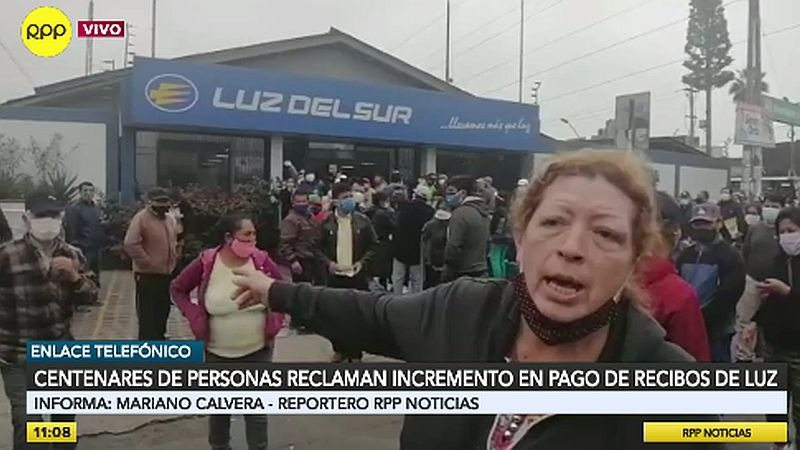
\includegraphics[width=.7\textwidth]{./Figures/motivacion.jpg}
%\caption{Noticias de la problemática en Lima Perú \protect\footnotemark.}
%\label{fig:noticia}
%end{figure}
%\vspace{1cm}
%\footnotetext{Imagen tomada de \url{https://rpp.pe/noticias/luz-del-sur}}

El organismo supervisor del estado recordó que en los casos donde la lectura del medidor confirme que el consumo real ha sido menor al facturado, la empresa deberá devolver lo pagado en exceso en una sola oportunidad o proceder a refacturar \citep{WEBSITE:2}.

Realizar el proceso de refacturación para corregir estos errores costará demasiado tiempo y dinero al estado y a las empresas que ofrecen dicho servicio, presentando incomodidad y daño económico a toda la población afectada. 

Como efecto de esta problemática en Perú, surge la necesidad de desarrollar un sistema de monitoreo y control que permita conocer el consumo eléctrico mensual detallado, siendo este una herramienta automatizada de respaldo y que sirva como evidencia para prevenir facturaciones erróneas para hogares, edificios habitacionales, empresas, etc.

%-----------------------------------------------------------------------



%----------------------------------------------------------------------------------------
\section{Propósito y alcance}



%\subsection{Propósito}

El propósito de este trabajo es diseñar y desarrollar un sistema prototipo operativo funcional capaz de controlar y monitorear viviendas u otros ambientes mediante el protocolo MQTT para brindar una gestión inteligente respecto a confort y consumo energético.

%\subsection{Alcance}

El alcance del proyecto incluye:
\begin{itemize}
\item Diseño y desarrollo de un módulo principal local.
\item Diseño y desarrollo del módulo replicador de datos local-nube.
\item Diseño y desarrollo del módulo actuador y de consumo eléctrico.
\item Diseño y desarrollo del módulo de control de temperatura.
\item Diseño y desarrollo de un \emph{software} web a medida para la gestión de control y monitoreo de una vivienda o edificio.
\end{itemize}

%\subsection{Objetivos}
%\begin{itemize}
%\item Diseñar y desarrollar un sistema IoT para medir el consumo eléctrico.
%\item Diseñar y desarrollar un sistema que no dependa de una conexión a Internet para su funcionamiento.
%\item Diseñar y desarrollar un \emph{software} a medida para la gestión de control y monitoreo de una vivienda o edificio.
%\item Diseñar e implementar módulos con comunicación Wi-Fi para el control y monitoreo de energía eléctrica.
%\end{itemize}

%----------------------------------------------------------------------------------------
\let\cleardoublepage\clearpage % para eliminar pagina en blanco siguiente